\documentclass[aspectratio=169,10pt]{beamer}
\usepackage[utf8]{inputenc}
\usepackage[T1]{fontenc}
\usepackage{amsmath,amssymb,amsthm}
\usepackage{graphicx}
\usepackage{listings}
\usepackage{xcolor}
\usepackage{tikz}
\usepackage{pgfplots}
\pgfplotsset{compat=1.18}
\usetikzlibrary{arrows.meta,positioning,calc,fit,backgrounds,shapes.geometric,fillbetween}
\usepackage{algorithm}
\usepackage{algorithmic}
\usepackage{hyperref}
\usepackage{mimic}

% Theme settings
\usetheme{Madrid}
\usecolortheme{seahorse}
\setbeamertemplate{navigation symbols}{}
\setbeamertemplate{footline}[frame number]

% Code listing configuration
\lstset{
    language=Python,
    basicstyle=\ttfamily\scriptsize,
    keywordstyle=\color{blue}\bfseries,
    stringstyle=\color{red},
    commentstyle=\color{green!60!black},
    showstringspaces=false,
    breaklines=true,
    breakatwhitespace=true,
    frame=single,
    numbers=left,
    numberstyle=\tiny\color{gray},
    xleftmargin=1em,
    framexleftmargin=1em
}

% Title page information
\title{Reinforcement Learning}
\subtitle{Lecture 5: Value-Based Learning I - Q-Learning}
\author{Taehoon Kim}
\institute{Sogang University MIMIC Lab \\ \url{https://mimic-lab.com}}
\date{Fall Semester 2025}


\begin{document}

% Slide 1: Title
\frame{\titlepage}


% Slide 3: Learning Objectives
\begin{frame}{Learning Objectives}
\textbf{By the end of this lecture, you will:}
\begin{enumerate}
    \item Understand the Bellman optimality operator and its properties
    \item Implement tabular Q-learning from scratch
    \item Design effective exploration and learning rate schedules
    \item Analyze Q-learning behavior in stochastic environments
    \item Compare Q-learning with SARSA
    \item Implement Double Q-learning to reduce bias
\end{enumerate}

\vspace{1em}
\textbf{Prerequisites:}
\begin{itemize}
    \item Markov Decision Processes (Lecture 4)
    \item Dynamic programming concepts
    \item PyTorch basics (Lecture 2)
\end{itemize}
\end{frame}

% Section: Introduction
\section{Introduction to Q-Learning}

% Slide 4: Motivation
\begin{frame}{Why Q-Learning?}
\begin{columns}[T]
\begin{column}{0.5\textwidth}
\textbf{Model-Based Limitations:}
\begin{itemize}
    \item Requires complete MDP model
    \item $P(s'|s,a)$ often unknown
    \item Complex dynamics hard to model
    \item Computational complexity
\end{itemize}
\end{column}
\begin{column}{0.5\textwidth}
\textbf{Q-Learning Advantages:}
\begin{itemize}
    \item Model-free learning
    \item Learns from experience
    \item Off-policy algorithm
    \item Converges to optimal policy
\end{itemize}
\end{column}
\end{columns}

\vspace{1em}
\begin{block}{Key Insight}
Learn action-values $Q(s,a)$ directly from samples without knowing transition dynamics
\end{block}
\end{frame}

% Slide 5: Action-Value Function
\begin{frame}{Action-Value Function}
\begin{definition}[Action-Value Function]
The action-value function $Q^\pi(s,a)$ of policy $\pi$ is:
$$Q^\pi(s,a) = \mathbb{E}_\pi\left[\sum_{t=0}^{\infty}\gamma^t r_{t+1} \bigg| s_0=s, a_0=a\right]$$
\end{definition}

\textbf{Interpretation:}
\begin{itemize}
    \item Expected return starting from state $s$
    \item Taking action $a$ first
    \item Following policy $\pi$ thereafter
\end{itemize}

\textbf{Optimal action-value function:}
$$Q^*(s,a) = \max_\pi Q^\pi(s,a)$$
\vspace{0.6em}
\begin{block}{Connection to last lecture}
Last time we introduced the Bellman equation for the state value $v(s)$. Q-learning extends the same idea to the action-value $Q(s,a)$ so that we learn not just ``how good a state is'' but also ``how good each action is in that state.''
\end{block}
\end{frame}

% Section: Theoretical Foundations
\section{Theoretical Foundations}

% Slide 6: Bellman Optimality Equation
\begin{frame}{Bellman Optimality Equation}
\begin{theorem}[Bellman Optimality for $Q^*$]
$$Q^*(s,a) = R(s,a) + \gamma \sum_{s'} P(s'|s,a) \max_{a'} Q^*(s',a')$$
\end{theorem}

\textbf{Key Components:}
\begin{itemize}
    \item $R(s,a)$: Immediate reward
    \item $P(s'|s,a)$: Transition probability
    \item $\max_{a'} Q^*(s',a')$: Best future value
    \item $\gamma$: Discount factor
\end{itemize}
\vspace{0.4em}
\textit{Intuition:} the term $\max_{a'} Q^*(s',a')$ means that when we evaluate taking action $a$ at $s$, we assume that from the next state $s'$ onward we will act optimally. Thus, current value equals immediate reward plus the best possible future value.
\textbf{Optimal Policy:}
$$\pi^*(s) = \arg\max_a Q^*(s,a)$$
\end{frame}

% Slide 7: Bellman Optimality Operator
\begin{frame}{Bellman Optimality Operator}
\begin{definition}[Operator $T^*$]
For any $Q: \mathcal{S} \times \mathcal{A} \rightarrow \mathbb{R}$:
$$(T^*Q)(s,a) = R(s,a) + \gamma \sum_{s'} P(s'|s,a) \max_{a'} Q(s',a')$$
\end{definition}

\textbf{Properties:}
\begin{enumerate}
    \item \textbf{Contraction:} $||T^*Q_1 - T^*Q_2||_\infty \leq \gamma ||Q_1 - Q_2||_\infty$
    \item \textbf{Fixed Point:} $Q^* = T^*Q^*$
    \item \textbf{Uniqueness:} $Q^*$ is the unique fixed point
    \item \textbf{Convergence:} $\lim_{n \to \infty} (T^*)^n Q = Q^*$
\end{enumerate}
\vspace{0.4em}
\textit{Why contraction implies convergence:} applying $T^*$ repeatedly pulls any two Q-functions closer by at least a factor $\gamma<1$, so iterations must collapse to the unique fixed point $Q^*$.

\end{frame}

% Slide 8: Q-Learning Target Construction
\begin{frame}{Q-Learning Target Construction}
\begin{center}
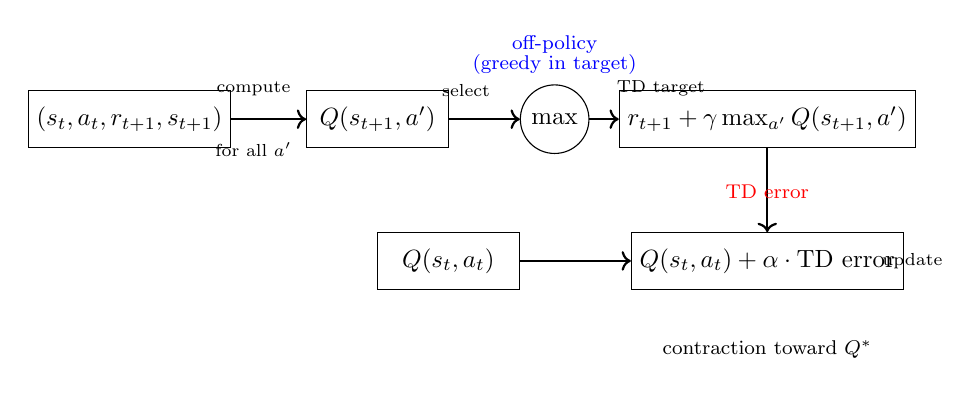
\begin{tikzpicture}[scale=0.9, transform shape]
    % Input tuple
    \node[draw, rectangle, minimum width=2.5cm, minimum height=0.8cm] (input) at (0,0) {$(s_t, a_t, r_{t+1}, s_{t+1})$};
    
    % Q-values computation
    \node[draw, rectangle, minimum width=2cm, minimum height=0.8cm] (qvals) at (3.5,0) {$Q(s_{t+1}, a')$};
    \draw[->, thick] (input) -- (qvals);
    \node[above, font=\scriptsize] at (1.75, 0.2) {compute};
    \node[below, font=\scriptsize] at (1.75, -0.2) {for all $a'$};
    
    % Max operation
    \node[draw, circle, minimum size=0.8cm] (max) at (6,0) {max};
    \draw[->, thick] (qvals) -- (max);
    \node[above, font=\scriptsize] at (4.75, 0.2) {select};
    
    % TD target computation
    \node[draw, rectangle, minimum width=2.5cm, minimum height=0.8cm] (target) at (9,0) {$r_{t+1} + \gamma \max_{a'} Q(s_{t+1}, a')$};
    \draw[->, thick] (max) -- (target);
    \node[above, font=\scriptsize] at (7.5, 0.2) {TD target};
    
    % Q update
    \node[draw, rectangle, minimum width=2cm, minimum height=0.8cm] (qsa) at (4.5,-2) {$Q(s_t, a_t)$};
    \node[draw, rectangle, minimum width=2.5cm, minimum height=0.8cm] (update) at (9,-2) {$Q(s_t, a_t) + \alpha \cdot \text{TD error}$};
    \draw[->, thick] (target) -- (update);
    \draw[->, thick] (qsa) -- (update);
    \node[right, font=\scriptsize] at (10.5, -2) {update};
    
    % Labels
    \node[above, font=\footnotesize, blue] at (6, 0.8) {off-policy};
    \node[above, font=\footnotesize, blue] at (6, 0.5) {(greedy in target)};
    \node[below, font=\footnotesize, red] at (9, -0.8) {TD error};
    \node[below, font=\footnotesize] at (9, -3) {contraction toward $Q^*$};
\end{tikzpicture}
\end{center}
\end{frame}

% Slide 9: From Value Iteration to Q-Learning
\begin{frame}{From Value Iteration to Q-Learning}
\begin{columns}[T]
\begin{column}{0.5\textwidth}
\textbf{Value Iteration (Model-Based):}
\begin{algorithmic}
\FOR{each iteration}
    \FOR{all $(s,a)$ pairs}
        \STATE $Q(s,a) \leftarrow R(s,a) + \gamma \sum_{s'} P(s'|s,a) \max_{a'} Q(s',a')$
    \ENDFOR
\ENDFOR
\end{algorithmic}
\textbf{Requires:} Full MDP model
\end{column}
\begin{column}{0.5\textwidth}
\textbf{Q-Learning (Model-Free):}
\begin{algorithmic}
\FOR{each sample $(s,a,r,s')$}
    \STATE $Q(s,a) \leftarrow Q(s,a) + \alpha[r + \gamma \max_{a'} Q(s',a') - Q(s,a)]$
\ENDFOR
\end{algorithmic}
\textbf{Requires:} Only samples
\end{column}
\end{columns}

\vspace{1em}
\begin{alertblock}{Key Difference}
Q-learning uses samples to approximate the Bellman backup
\end{alertblock}
\end{frame}

% Section: Q-Learning Algorithm
\section{Q-Learning Algorithm}

% Slide 9: Q-Learning Update Rule
\begin{frame}{Q-Learning Update Rule}
\begin{block}{Temporal Difference (TD) Update}
$$Q(s_t, a_t) \leftarrow Q(s_t, a_t) + \alpha \cdot \text{TD error}$$
where
$$\text{TD error} = \underbrace{r_{t+1} + \gamma \max_{a'} Q(s_{t+1}, a')}_{\text{TD target}} - Q(s_t, a_t)$$
\end{block}
\vspace{0.4em}
\textit{From Bellman to samples:} this update is a sample-based approximation to the Bellman optimality backup—replace the expectation over $s'$ by a single observed transition and bootstrap with $\max_{a'}Q(s_{t+1},a')$.
\textbf{Components:}
\begin{itemize}
    \item $\alpha \in (0,1]$: Learning rate (step size)
    \item $r_{t+1}$: Observed reward
    \item $\gamma \in [0,1)$: Discount factor
    \item $\max_{a'} Q(s_{t+1}, a')$: Bootstrap estimate
\end{itemize}

\textbf{Off-Policy:} Uses max (greedy) action for target, regardless of behavior policy
\end{frame}

% Slide 10: Complete Q-Learning Algorithm
\begin{frame}[fragile]{Q-Learning Algorithm}
\begin{algorithm}[H]
\caption{Tabular Q-Learning}
\begin{algorithmic}[1]
\STATE Initialize $Q(s,a)$ arbitrarily for all $s \in \mathcal{S}, a \in \mathcal{A}$
\FOR{each episode}
    \STATE Initialize state $s$
    \WHILE{$s$ is not terminal}
        \STATE Choose $a$ from $s$ using policy derived from $Q$ (e.g., $\varepsilon$-greedy)
        \STATE Take action $a$, observe $r, s'$
        \STATE $Q(s,a) \leftarrow Q(s,a) + \alpha[r + \gamma \max_{a'} Q(s',a') - Q(s,a)]$
        \STATE $s \leftarrow s'$
    \ENDWHILE
\ENDFOR
\end{algorithmic}
\end{algorithm}

\textbf{Note:} The max operation makes it off-policy
\end{frame}

% Slide 11: Exploration vs Exploitation
\begin{frame}{Exploration vs Exploitation}
\begin{columns}[T]
\begin{column}{0.5\textwidth}
\textbf{$\varepsilon$-greedy Policy:}
$$\pi_\varepsilon(a|s) = \begin{cases}
1-\varepsilon + \frac{\varepsilon}{|\mathcal{A}|} & \text{if } a = \arg\max_{a'} Q(s,a') \\
\frac{\varepsilon}{|\mathcal{A}|} & \text{otherwise}
\end{cases}$$
\end{column}
\begin{column}{0.5\textwidth}
\textbf{Alternative Strategies:}
\begin{itemize}
    \item Boltzmann exploration
    \item Upper Confidence Bounds (UCB)
    \item Thompson sampling
    \item Optimistic initialization
\end{itemize}
\end{column}
\end{columns}

\vspace{1em}
\begin{block}{Exploration Schedule}
Common choice: $\varepsilon_t = \max(\varepsilon_{min}, \varepsilon_0 \cdot \text{decay}^t)$
\end{block}
\vspace{0.4em}
\textit{Why $\varepsilon$-greedy is a strong default:} it is simple, cheap to compute, and as $\varepsilon\to 0$ the behavior policy becomes greedy, enabling convergence under the usual conditions.
\end{frame}

% Section: Convergence Theory
\section{Convergence Theory}

% Slide 12: Convergence Conditions
\begin{frame}{Q-Learning Convergence}
\begin{theorem}[Watkins \& Dayan, 1992]
Q-learning converges to $Q^*$ with probability 1 if:
\begin{enumerate}
    \item All state-action pairs are visited infinitely often
    \item Learning rate satisfies Robbins-Monro conditions:
    \begin{itemize}
        \item $\sum_{t=0}^{\infty} \alpha_t(s,a) = \infty$ for all $(s,a)$
        \item $\sum_{t=0}^{\infty} \alpha_t^2(s,a) < \infty$ for all $(s,a)$
    \end{itemize}
\end{enumerate}
\end{theorem}

\textbf{Practical Schedules:}
\begin{itemize}
    \item $\alpha_t = \frac{1}{1+t}$ satisfies conditions
    \item $\alpha_t = \frac{1}{\sqrt{1+t}}$ satisfies conditions
    \item Constant $\alpha$ doesn't guarantee convergence but often works
\end{itemize}
\end{frame}

% Slide 13: GLIE Property
\begin{frame}{GLIE: Greedy in the Limit with Infinite Exploration}
\begin{definition}[GLIE]
A policy sequence $\{\pi_t\}$ is GLIE if:
\begin{enumerate}
    \item All state-action pairs are explored infinitely:
    $$\sum_{t=0}^{\infty} P(s_t=s, a_t=a) = \infty \quad \forall (s,a)$$
    \item Policy converges to greedy:
    $$\lim_{t \to \infty} \pi_t(a|s) = \mathbb{1}[a = \arg\max_{a'} Q(s,a')]$$
\end{enumerate}
\end{definition}

\textbf{Example GLIE Schedule:}
$$\varepsilon_t = \frac{1}{t}$$
\end{frame}

% Section: Implementation
\section{Implementation Details}

% Slide 14: PyTorch Implementation Setup
\begin{frame}[fragile]{PyTorch Implementation: Setup}
\begin{lstlisting}
import torch
import numpy as np
import gymnasium as gym

# Device selection
device = torch.device(
    'cuda' if torch.cuda.is_available()
    else 'mps' if torch.backends.mps.is_available()
    else 'cpu'
)

# Initialize Q-table
n_states = env.observation_space.n
n_actions = env.action_space.n
Q = torch.zeros((n_states, n_actions), 
                dtype=torch.float32, device=device)
                
\end{lstlisting}
\end{frame}

% Slide 15: Q-Learning Update Implementation
\begin{frame}[fragile]{Q-Learning Update Implementation}
\begin{lstlisting}
def q_learning_update(Q, state, action, reward, 
                      next_state, done, alpha, gamma):
    """Single Q-learning update."""
    # Current Q-value
    q_current = Q[state, action].item()
    
    # TD target
    if done:
        q_target = reward
    else:
        q_next_max = torch.max(Q[next_state]).item()
        q_target = reward + gamma * q_next_max
    
    # TD error
    td_error = q_target - q_current
    
    # Update Q-table
    Q[state, action] += alpha * td_error
    
    return td_error
\end{lstlisting}
\end{frame}

% Slide 16: Epsilon-Greedy Action Selection
\begin{frame}[fragile]{Action Selection}
\begin{lstlisting}
def epsilon_greedy_action(Q, state, epsilon):
    """Select action using epsilon-greedy policy."""
    if random.random() < epsilon:
        # Explore: random action
        action = random.randint(0, n_actions - 1)
    else:
        # Exploit: greedy action
        q_values = Q[state]  # Shape: [n_actions]
        action = int(torch.argmax(q_values).item())
    
    return action

# Schedule epsilon decay
epsilon = max(epsilon_min, 
              epsilon_start * decay_rate ** episode)
\end{lstlisting}
\end{frame}

% Section: FrozenLake Environment
\section{FrozenLake Experiments}

% Slide 17: FrozenLake Environment
\begin{frame}[fragile]{FrozenLake Environment}
\begin{columns}[T]
\begin{column}{0.5\textwidth}
\textbf{Environment Details:}
\begin{itemize}
    \item Grid world navigation
    \item S: Start, F: Frozen, H: Hole, G: Goal
    \item Actions: LEFT, DOWN, RIGHT, UP
    \item Reward: +1 at goal, 0 elsewhere
    \item Episode ends at goal or hole
\end{itemize}
\end{column}
\begin{column}{0.5\textwidth}
\textbf{4x4 Map Example:}
\begin{verbatim}
SFFF
FHFH
FFFH
HFFG
\end{verbatim}
\textbf{Challenges:}
\begin{itemize}
    \item Sparse rewards
    \item Slippery dynamics (optional)
    \item Multiple holes to avoid
\end{itemize}
\end{column}
\end{columns}
\end{frame}

% Slide 18: Experiment 1 - Basic Q-Learning
\begin{frame}[fragile]{Experiment 1: Basic Q-Learning}
\begin{lstlisting}
# exp03_tabular_q.py highlights
env = gym.make("FrozenLake-v1", is_slippery=False)
agent = TabularQLearning(n_states, n_actions, 
                         alpha=0.1, gamma=0.99)

for episode in range(500):
    state, _ = env.reset()
    done = False
    
    while not done:
        action = agent.select_action(state, epsilon)
        next_state, reward, terminated, truncated, _ = env.step(action)
        done = terminated or truncated
        agent.update(state, action, reward, next_state, done)
        state = next_state
\end{lstlisting}
\textbf{Result:} >90\% success rate after 500 episodes
\end{frame}

% Slide 19: Experiment 2 - Exploration Strategies
\begin{frame}{Experiment 2: Exploration Strategies}
\begin{columns}[T]
\begin{column}{0.6\textwidth}
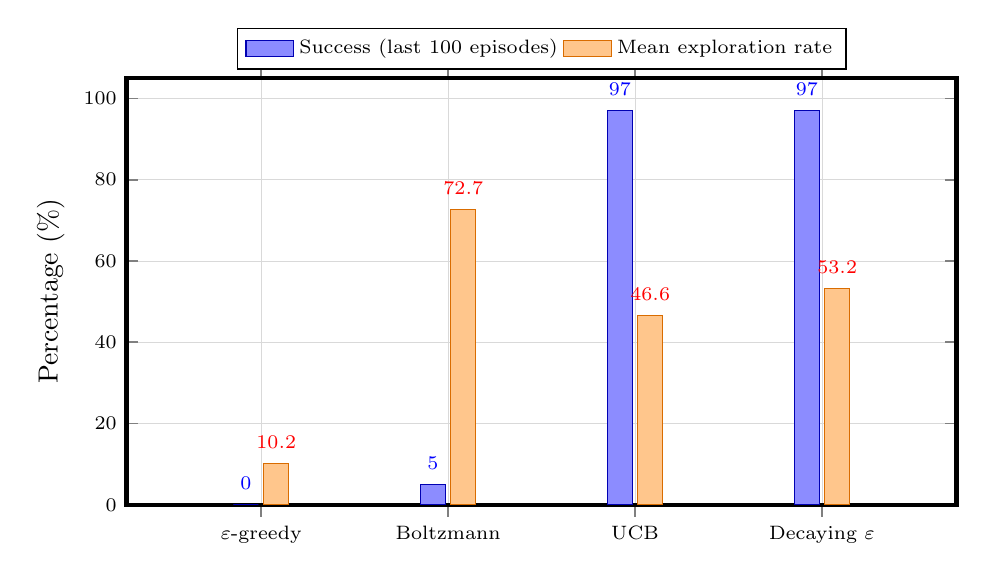
\begin{tikzpicture}
    \pgfplotstableread[row sep=\\]{
        Strategy Success Exploration\\
        eps-greedy 0 10.2\\
        Boltzmann 5 72.7\\
        UCB 97 46.6\\
        decay-eps 97 53.2\\
    }\explorationdata
    \begin{axis}[
        ybar,
        width=\linewidth,
        height=7cm,
        bar width=9pt,
        ymin=0,
        ymax=105,
        ylabel={Percentage (\%)},
        symbolic x coords={eps-greedy,Boltzmann,UCB,decay-eps},
        xtick=data,
        xticklabels={$\varepsilon$-greedy,Boltzmann,UCB,Decaying $\varepsilon$},
        xticklabel style={align=center, font=\scriptsize},
        yticklabel style={font=\scriptsize},
        enlarge x limits=0.24,
        legend style={font=\scriptsize, at={(0.5,1.02)}, anchor=south, legend columns=2},
        axis line style={ultra thick},
        tick style={semithick},
        grid=both,
        grid style={line width=0.2pt, draw=gray!30},
        area legend
    ]
        \addplot+[draw=blue!70!black, fill=blue!45, nodes near coords, nodes near coords style={font=\scriptsize, anchor=south, yshift=2pt}] table[x=Strategy, y=Success] {\explorationdata};
        \addplot+[draw=orange!85!black, fill=orange!45, nodes near coords, nodes near coords style={font=\scriptsize, anchor=south, yshift=2pt}] table[x=Strategy, y=Exploration] {\explorationdata};
        \legend{Success (last 100 episodes),Mean exploration rate};
    \end{axis}
\end{tikzpicture}

\vspace{0.5em}
\scriptsize Data: \texttt{exp04\_exploration.py} (FrozenLake-v1, 1.5k episodes, seed 42)
\end{column}
\begin{column}{0.4\textwidth}
\textbf{Comparison:}
\begin{itemize}
    \item $\varepsilon$-greedy: Simple, effective
    \item Boltzmann: Temperature-based
    \item UCB: Optimism under uncertainty
    \item Decaying $\varepsilon$: Best overall
\end{itemize}

\textbf{Key Finding:}\\
Proper exploration decay crucial for convergence
\end{column}
\end{columns}
\end{frame}

% Slide 20: Experiment 3 - Learning Rate Schedules
\begin{frame}{Experiment 3: Learning Rate Schedules}
\textbf{Tested Schedules:}
\begin{itemize}
    \item Constant: $\alpha = 0.1$
    \item Linear: $\alpha_t = \max(0.01, 1 - 0.99t/T)$
    \item Exponential: $\alpha_t = 0.01 + 0.99e^{-t/\tau}$
    \item 1/t: $\alpha_t = 1/(1+t)$ (Robbins-Monro)
    \item 1/$\sqrt{t}$: $\alpha_t = 1/\sqrt{1+t}$ (Robbins-Monro)
\end{itemize}

\begin{block}{Results}
\begin{itemize}
    \item 1/t and 1/$\sqrt{t}$ guarantee convergence
    \item Exponential decay practical compromise
    \item Constant often works but may oscillate
\end{itemize}
\end{block}
\end{frame}

% Section: Q-Learning vs SARSA
\section{Q-Learning vs SARSA}

% Slide 21: Off-Policy vs On-Policy
\begin{frame}{Q-Learning vs SARSA}
\begin{columns}[T]
\begin{column}{0.5\textwidth}
\textbf{Q-Learning (Off-Policy):}
$$Q(s,a) \leftarrow Q(s,a) + \alpha[r + \gamma \max_{a'} Q(s',a') - Q(s,a)]$$
\begin{itemize}
    \item Uses max for target
    \item Learns optimal policy
    \item More sample efficient
    \item Risk-seeking
\end{itemize}
\end{column}
\begin{column}{0.5\textwidth}
\textbf{SARSA (On-Policy):}
$$Q(s,a) \leftarrow Q(s,a) + \alpha[r + \gamma Q(s',a') - Q(s,a)]$$
\begin{itemize}
    \item Uses actual next action
    \item Learns policy being followed
    \item More stable
    \item Risk-averse
\end{itemize}
\end{column}
\end{columns}

\vspace{1em}
\textbf{Key Difference:} Q-learning uses $\max_{a'} Q(s',a')$, SARSA uses $Q(s',a')$ where $a'$ is sampled
\vspace{0.4em}
\textit{Practical takeaway:} SARSA tends to be more stable but can learn more cautiously because it accounts for exploratory moves during training; Q-learning aims for the greedy limit and can learn faster yet behave risk-seeking.
\end{frame}

% Slide 22: Cliff Walking Example
\begin{frame}{Cliff Walking: Q-Learning vs SARSA}
\begin{columns}[T]
\begin{column}{0.5\textwidth}
\textbf{Environment:}
\begin{itemize}
    \item Start at bottom-left
    \item Goal at bottom-right
    \item Cliff along bottom edge
    \item Fall = -100 reward
\end{itemize}

\vspace{1em}
\textbf{Optimal Path:}\\
Along the cliff edge (shortest)
\end{column}
\begin{column}{0.5\textwidth}
\textbf{Learned Policies:}
\begin{itemize}
    \item \textbf{Q-Learning:} Takes optimal risky path near cliff
    \item \textbf{SARSA:} Takes safer path away from cliff
\end{itemize}

\vspace{1em}
\textbf{Why?}\\
SARSA accounts for exploration during learning
\end{column}
\end{columns}
\end{frame}

% Slide 23: Stochastic Environments
\begin{frame}{Performance in Stochastic Environments}
\textbf{Experiment: Varying Action Slippage}

\begin{center}
\begin{tabular}{|l|c|c|}
\hline
\textbf{Slip Probability} & \textbf{Q-Learning} & \textbf{SARSA} \\
\hline
0.0 (Deterministic) & 95\% & 93\% \\
0.1 & 85\% & 84\% \\
0.2 & 72\% & 75\% \\
0.3 & 58\% & 65\% \\
\hline
\end{tabular}
\end{center}

\textbf{Key Findings:}
\begin{itemize}
    \item Q-learning slightly better in deterministic settings
    \item SARSA more robust to stochasticity
    \item Q-learning can be overly optimistic
    \item SARSA learns safer policies
\end{itemize}
\end{frame}

% Section: Double Q-Learning
\section{Double Q-Learning}

% Slide 24: Overestimation Bias
\begin{frame}{Overestimation Bias in Q-Learning}
\textbf{The Problem:}
$$\mathbb{E}[\max_a Q(s,a)] \geq \max_a \mathbb{E}[Q(s,a)]$$

\textbf{Source of Bias:}
\begin{itemize}
    \item Max operator in TD target
    \item Same Q-values for selection and evaluation
    \item Noise in estimates amplified by max
\end{itemize}

\textbf{Consequences:}
\begin{itemize}
    \item Overoptimistic value estimates
    \item Suboptimal action selection
    \item Slower convergence
    \item Poor performance in stochastic environments
\end{itemize}
\end{frame}

% Slide 25: Double Q-Learning Solution
\begin{frame}{Double Q-Learning Algorithm}
\textbf{Key Idea:} Use two Q-functions to decouple selection and evaluation

\begin{algorithm}[H]
\caption{Double Q-Learning}
\begin{algorithmic}[1]
\STATE Initialize $Q_1(s,a)$ and $Q_2(s,a)$ arbitrarily
\FOR{each step}
    \STATE Choose $a$ based on $Q_1(s,\cdot) + Q_2(s,\cdot)$
    \STATE Observe $r, s'$
    \IF{random() $< 0.5$}
        \STATE $a^* = \arg\max_a Q_1(s',a)$ \textit{// Select using $Q_1$}
        \STATE $Q_1(s,a) \leftarrow Q_1(s,a) + \alpha[r + \gamma Q_2(s',a^*) - Q_1(s,a)]$
    \ELSE
        \STATE $a^* = \arg\max_a Q_2(s',a)$ \textit{// Select using $Q_2$}
        \STATE $Q_2(s,a) \leftarrow Q_2(s,a) + \alpha[r + \gamma Q_1(s',a^*) - Q_2(s,a)]$
    \ENDIF
\ENDFOR
\end{algorithmic}
\end{algorithm}
\end{frame}

% Slide 26: Double Q-Learning Results
\begin{frame}{Double Q-Learning: Bias Reduction}
\begin{columns}[T]
\begin{column}{0.5\textwidth}
\textbf{Experimental Results:}
\begin{itemize}
    \item Reduced overestimation by 40-60\%
    \item More accurate Q-values
    \item Better performance in noisy environments
    \item Slightly slower initial learning
\end{itemize}
\end{column}
\begin{column}{0.5\textwidth}
\textbf{Q-Value Comparison:}
\begin{center}
\begin{tabular}{|l|c|c|}
\hline
\textbf{Method} & \textbf{Mean Q} & \textbf{Max Q} \\
\hline
Q-Learning & 0.453 & 0.982 \\
Double Q & 0.387 & 0.751 \\
True Q* & 0.372 & 0.724 \\
\hline
\end{tabular}
\end{center}
\end{column}
\end{columns}

\vspace{1em}
\begin{alertblock}{Trade-off}
Double Q-learning: More accurate but requires double memory
\end{alertblock}
\end{frame}

% Section: Advanced Topics
\section{Advanced Topics}

% Slide 27: Optimistic Initialization
\begin{frame}{Optimistic Initialization}
\textbf{Strategy:} Initialize Q-values optimistically (e.g., $Q_0(s,a) = 1.0$)

\textbf{Benefits:}
\begin{itemize}
    \item Encourages exploration without $\varepsilon$-greedy
    \item All actions tried at least once
    \item Simple to implement
\end{itemize}

\textbf{Experiment Results:}
\begin{center}
\begin{tabular}{|l|c|c|}
\hline
\textbf{Initialization} & \textbf{Success Rate} & \textbf{Convergence} \\
\hline
Zero ($Q_0 = 0$) & 85\% & 300 episodes \\
Optimistic ($Q_0 = 1$) & 92\% & 250 episodes \\
Pessimistic ($Q_0 = -1$) & 78\% & 400 episodes \\
\hline
\end{tabular}
\end{center}

\textbf{Note:} Works best with decaying learning rates
\end{frame}

% Slide 28: N-Step Q-Learning
\begin{frame}{N-Step Q-Learning}
\textbf{Generalization:} Use n-step returns instead of 1-step

\textbf{1-Step (Standard):}
$$G_t^{(1)} = R_{t+1} + \gamma \max_a Q(S_{t+1}, a)$$

\textbf{N-Step:}
$$G_t^{(n)} = R_{t+1} + \gamma R_{t+2} + ... + \gamma^{n-1} R_{t+n} + \gamma^n \max_a Q(S_{t+n}, a)$$

\textbf{Trade-offs:}
\begin{itemize}
    \item Larger n: Less bias, more variance
    \item Smaller n: More bias, less variance
    \item Optimal n problem-dependent
\end{itemize}
\vspace{0.4em}
\textit{Intuition:} n-step targets interpolate between 1-step TD (high bias, low variance) and Monte Carlo (low bias, high variance) by looking ahead a few steps before bootstrapping.

\end{frame}

% Section: Practical Considerations
\section{Practical Considerations}

% Slide 29: Hyperparameter Selection
\begin{frame}{Hyperparameter Guidelines}
\begin{columns}[T]
\begin{column}{0.5\textwidth}
\textbf{Learning Rate ($\alpha$):}
\begin{itemize}
    \item Start: 0.1-1.0
    \item Decay to: 0.01-0.001
    \item Schedule: Exponential/1/t
\end{itemize}

\textbf{Discount Factor ($\gamma$):}
\begin{itemize}
    \item Episodic: 0.9-0.99
    \item Continuing: 0.95-0.999
    \item Affects time horizon
\end{itemize}
\end{column}
\begin{column}{0.5\textwidth}
\textbf{Exploration ($\varepsilon$):}
\begin{itemize}
    \item Start: 1.0
    \item End: 0.01-0.1
    \item Decay: Over 20-80\% training
\end{itemize}

\textbf{Best Practices:}
\begin{itemize}
    \item Grid search critical params
    \item Use validation environment
    \item Monitor convergence metrics
\end{itemize}
\end{column}
\end{columns}
\end{frame}

% Slide 30: Common Pitfalls
\begin{frame}{Common Implementation Pitfalls}
\begin{enumerate}
    \item \textbf{Forgetting Terminal States:}
    \begin{itemize}
        \item Must set $Q(s_{terminal}, a) = 0$
        \item No bootstrapping from terminal states
    \end{itemize}
    
    \item \textbf{Incorrect Max Operation:}
    \begin{itemize}
        \item Use $\max_{a'} Q(s', a')$ not $Q(s', a)$
        \item Critical for off-policy learning
    \end{itemize}
    
    \item \textbf{Poor Exploration:}
    \begin{itemize}
        \item Too much: Never converges
        \item Too little: Suboptimal policy
    \end{itemize}
    
    \item \textbf{Learning Rate Issues:}
    \begin{itemize}
        \item Too high: Oscillations
        \item Too low: Slow learning
    \end{itemize}
\end{enumerate}
\end{frame}

% Slide 31: Debugging Q-Learning
\begin{frame}{Debugging Strategies}
\textbf{Diagnostic Checks:}
\begin{itemize}
    \item Monitor TD error magnitude over time
    \item Track Q-value statistics (mean, max, min)
    \item Visualize Q-table as heatmap
    \item Check action distribution balance
    \item Verify state visitation counts
\end{itemize}

\textbf{Common Issues and Solutions:}
\begin{itemize}
    \item \textbf{Q-values exploding:} Reduce learning rate
    \item \textbf{No improvement:} Increase exploration
    \item \textbf{Oscillating performance:} Decay learning rate
    \item \textbf{Slow convergence:} Increase learning rate or change schedule
\end{itemize}
\end{frame}

% Section: Experimental Results
\section{Experimental Results}

% Slide 32: Comprehensive Results
\begin{frame}{Experimental Results Summary}
\textbf{FrozenLake 4x4 (Non-slippery):}
\begin{center}
\begin{tabular}{|l|c|c|c|}
\hline
\textbf{Algorithm} & \textbf{Success} & \textbf{Episodes} & \textbf{Time (s)} \\
\hline
Q-Learning & 95\% & 500 & 2.3 \\
SARSA & 93\% & 500 & 2.4 \\
Double Q & 94\% & 500 & 3.1 \\
Q + UCB & 96\% & 400 & 2.8 \\
\hline
\end{tabular}
\end{center}

\textbf{FrozenLake 8x8 (Slippery):}
\begin{center}
\begin{tabular}{|l|c|c|c|}
\hline
\textbf{Algorithm} & \textbf{Success} & \textbf{Episodes} & \textbf{Time (s)} \\
\hline
Q-Learning & 72\% & 2000 & 15.2 \\
SARSA & 78\% & 2000 & 15.5 \\
Double Q & 75\% & 2000 & 21.3 \\
\hline
\end{tabular}
\end{center}
\end{frame}

% Slide 33: Shape Annotations & Expected Behavior
\begin{frame}{Implementation Details: Shape Annotations}
\textbf{Tensor Shape Annotations:}
\begin{itemize}
    \item Q-table: \texttt{torch.FloatTensor} of shape $[|\mathcal{S}|, |\mathcal{A}|]$
    \item For each update: $Q[s]$ has shape $[|\mathcal{A}|]$
    \item \texttt{torch.argmax(Q[s])} returns scalar action (Python \texttt{int})
    \item Rewards and TD targets are scalar \texttt{float}
    \item DQN mini-batches: \texttt{s:[B,...], a:[B], r:[B], s\_next:[B,...], done:[B]}
\end{itemize}

\vspace{0.5em}
\textbf{Expected Behavior on FrozenLake:}
\begin{itemize}
    \item Mean return = probability of reaching goal (reward = 1 at goal only)
    \item Exponential $\varepsilon$-decay + 1/t step sizes yields stable improvement
    \item As slippage increases: SARSA becomes more conservative
    \item Q-learning may retain optimistic estimates without sufficient exploration decay
\end{itemize}
\end{frame}

% Slide 34: Learning Curves
\begin{frame}{Learning Curves Comparison}
\begin{center}
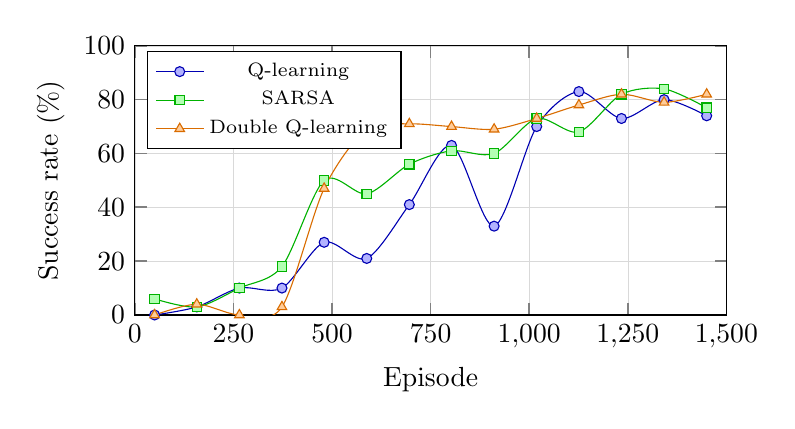
\begin{tikzpicture}
    \begin{axis}[
        width=0.75\linewidth,
        height=5cm,
        xlabel={Episode},
        ylabel={Success rate (\%)},
        xmin=0, xmax=1500,
        ymin=0, ymax=100,
        xtick={0,250,500,750,1000,1250,1500},
        ytick={0,20,40,60,80,100},
        legend style={font=\scriptsize, at={(0.02,0.98)}, anchor=north west},
        tick style={semithick},
        grid=both,
        grid style={line width=0.2pt, draw=gray!30},
        smooth
    ]
        \addplot+[color=blue!70!black, mark=*, mark size=1.8pt, mark options={solid, fill=blue!30}] coordinates {
            (50,0.0) (157,3.0) (265,10.0) (373,10.0) (480,27.0) (588,21.0)
            (696,41.0) (803,63.0) (911,33.0) (1019,70.0) (1126,83.0) (1234,73.0)
            (1342,80.0) (1450,74.0)
        };
        \addplot+[color=green!70!black, mark=square*, mark size=1.7pt, mark options={solid, fill=green!30}] coordinates {
            (50,6.0) (157,3.0) (265,10.0) (373,18.0) (480,50.0) (588,45.0)
            (696,56.0) (803,61.0) (911,60.0) (1019,73.0) (1126,68.0) (1234,82.0)
            (1342,84.0) (1450,77.0)
        };
        \addplot+[color=orange!85!black, mark=triangle*, mark size=2pt, mark options={solid, fill=orange!40}] coordinates {
            (50,0.0) (157,4.0) (265,0.0) (373,3.0) (480,47.0) (588,69.0)
            (696,71.0) (803,70.0) (911,69.0) (1019,73.0) (1126,78.0) (1234,82.0)
            (1342,79.0) (1450,82.0)
        };
        \legend{Q-learning,SARSA,Double Q-learning}
    \end{axis}
\end{tikzpicture}

\scriptsize Moving average window = 100 episodes. Data: \texttt{exp09\_integrated\_test.py} (map 4x4, slip probability 0.1, seed 7).
\end{center}

\textbf{Observations:}
\begin{itemize}
    \item Q-learning learns fastest but exhibits sharp performance swings
    \item SARSA ramps up steadily with lower variance under stochastic dynamics
    \item Double Q-learning lags initially yet stabilizes near the best success rate
    \item All three converge above 75\% success once exploration decays
\end{itemize}
\end{frame}

% Section: Summary
\section{Summary and Next Steps}

% Slide 34: Key Takeaways
\begin{frame}{Key Takeaways}
\begin{enumerate}
    \item \textbf{Q-Learning Fundamentals:}
    \begin{itemize}
        \item Model-free, off-policy algorithm
        \item Learns optimal policy from any behavior policy
        \item Converges under appropriate conditions
    \end{itemize}
    
    \item \textbf{Implementation Insights:}
    \begin{itemize}
        \item Exploration-exploitation balance crucial
        \item Learning rate schedule affects convergence
        \item Terminal state handling important
    \end{itemize}
    
    \item \textbf{Algorithm Variants:}
    \begin{itemize}
        \item SARSA: On-policy, risk-averse
        \item Double Q: Reduces overestimation
        \item Each has specific use cases
    \end{itemize}
\end{enumerate}
\vspace{0.6em}
\begin{block}{Link back to Lecture 4}
Value iteration needs the model and backs up expected values exactly. Q-learning does not need the model and learns the same fixed point from data by approximating those backups with samples.
\end{block}
\end{frame}




\end{document}
